\section{Experiment}
    \subsection{Data Preprocessing}
        \begin{figure}[tbh]
            \centering
            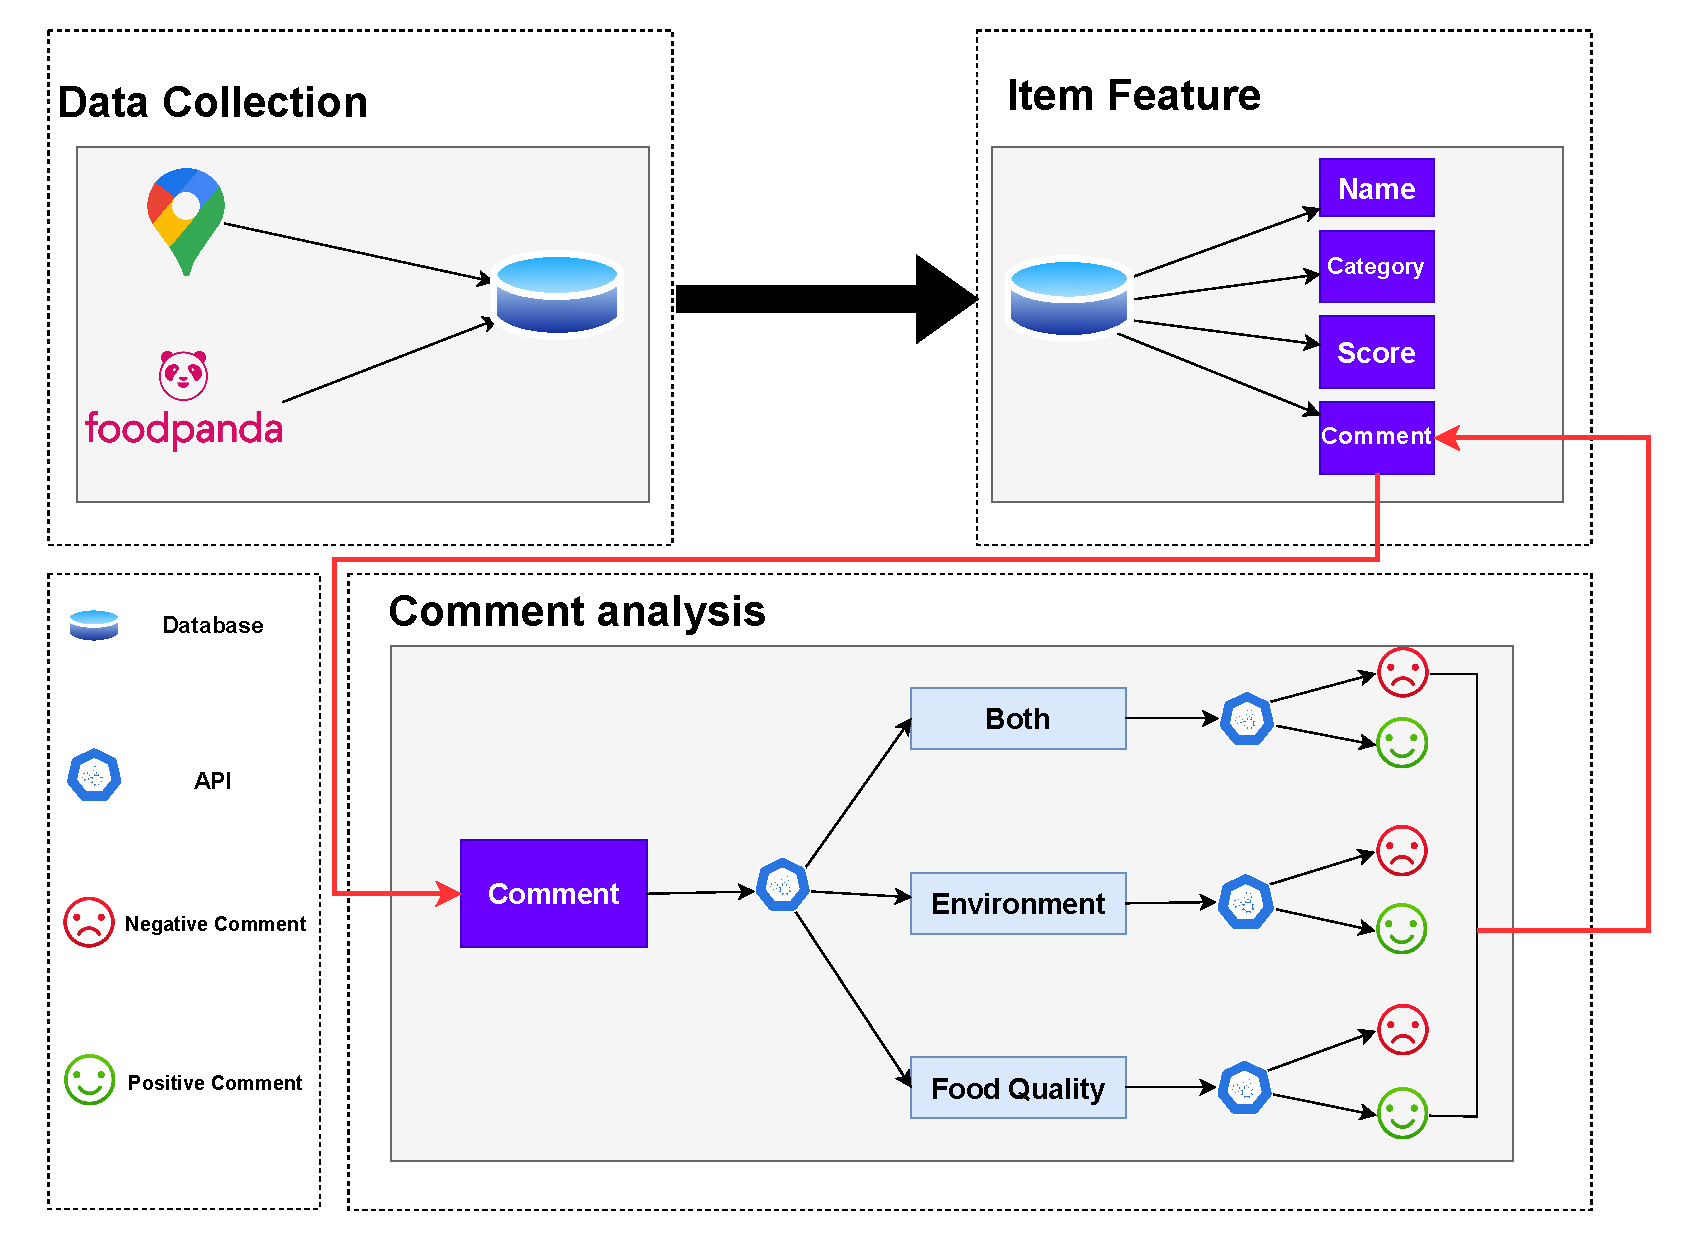
\includegraphics[width=0.5\textwidth]{img/preprocess.pdf}
            \caption{資料前處理架構圖}
            \label{fig-preprocess}
        \end{figure}
        本研究的資料前處理架構如 \textbackslash xfig\{fig-preprocess\} 所示,透過爬蟲技術從 Foodpanda 與 Google Maps 收集餐廳相關資料。每間餐廳的數據包含餐廳名稱、類型、評分以及顧客評論。由於餐廳通常會累積大量評論,這些評論對於描述店家的服務品質、餐點特色與顧客體驗具有高度相關性。然而,若將所有評論直接整合後丟入 GPT-4 進行分析,評論主題的多樣性可能導致資訊雜亂,進而影響模型微調(fine-tuning)的效果。當不同主題的評論混合訓練時,模型可能難以準確識別每類特徵的意圖,進一步降低結果的精確性。

        為解決上述問題並提升模型的針對性,本研究先將評論依主題分為三類:\textbf{餐點品質}、\textbf{店內環境氛圍},以及\textbf{綜合評價}。針對這三類評論,分別進行獨立的 LLM 微調,以使每個模型專注於特定主題特徵,避免不同主題資訊的相互干擾。對於餐點品質的評論,模型學習重點為食物的口感、品質及外觀呈現;對於店內環境氛圍的評論,模型則專注於用餐環境、設計風格及舒適度的相關描述;而綜合評價的模型則著重於顧客的整體體驗。透過分主題進行微調,模型得以精準掌握各主題的特徵表現,進一步增強評論處理的針對性。
        \color{blue}
        完成主題分類及模型微調後,本研究針對各主題的評論進行情感分析,以判斷評論的情感取向(正面或負面)。主題分類與情感分類的結果分別以 one-hot encoding 表示。其中,主題分類的向量表示為:
        \begin{equation}
            \mathbf{h}_c \in \mathbb{R}^3,
        \end{equation}
        其三個維度分別對應於餐點品質 (\(c_1\))、店內環境氛圍 (\(c_2\)) 以及綜合評價 (\(c_3\))。情感分類的向量表示為:
        \begin{equation}
            \mathbf{h}_s \in \mathbb{R}^2,
        \end{equation}
        其中兩個維度分別對應正面情感(\(P\))與負面情感(\(N\))。將主題分類與情感分類的 one-hot encoding 串接後,得到評論的最終向量表示:
        \begin{equation}
            \mathbf{h_{i,j}} = [\mathbf{h}_c; \mathbf{h}_s] \in \mathbb{R}^5,
        \end{equation}
        其中 \([\cdot; \cdot]\) 表示向量的串接操作,\(\mathbf{h_{i,j}}\) 代表第 \(i\) 家餐廳中第 \(j\) 條評論的綜合向量表示。
        
        假設某店家 \(i\) 有 \(n_i\) 條評論,且每條評論 \(j\) 的嵌入向量為 \(\mathbf{h}_{i,j}\),本研究為評論賦予基於主題分類的權重 \(w(c_{i,j})\),其設定如下:
        \begin{equation}
            w(c) =
            \begin{cases}
            w_{1}, & \text{若 } c = c_1, \\
            w_{2}, & \text{若 } c = c_2, \\
            w_{3}, & \text{若 } c = c_3,
            \end{cases}
        \end{equation}
        最終,將所有評論的嵌入向量進行加權平均,以生成餐廳級別的嵌入向量:
        \begin{equation}
            \mathbf{h_i} = \frac{\sum_{j=1}^{n_i} w(c_{i,j}) \cdot \mathbf{h}_{i,j}}{n_i},
        \end{equation}
        其中 \(\mathbf{e_i}\) 表示店家 \(i\) 的最終評論嵌入向量,涵蓋該店所有評論的綜合信息,以上方法有效結合主題分類與情感分析,通過嵌入向量表示提升了餐廳評論處理的精確性與針對性,最後再將該向量乘上店家的評分,得到最終的餐廳嵌入向量,如下式所示:
        \begin{equation}
            \mathbf{e_i} = \mathbf{e_i} \times S_i,
        \end{equation}
        其中 \(S_i\) 代表店家 \(i\) 的評分,\(\mathbf{h_i}\) 為店家 \(i\) 的最終嵌入向量。
        


    \subsection{Dataset}
        \begin{table}[h]
            \centering
            \caption{\\ 數據集的統計分析}
            \begin{tabular}{lllll}
            \toprule
            \textbf{Dataset Name} & \textbf{User} & \textbf{Item} & \textbf{Interaction} & \textbf{Density} \\
            \hline
            Ratio 0.6 & 47 & 174 & 820 & 0.10026 \\
            \hline
            Ratio 0.7 & 47 & 174 & 957 & 0.11702 \\
            \hline
            Ratio 0.8 & 47 & 174 & 1115 & 0.13634 \\
            \hline
            Ratio 0.9 & 47 & 174 & 1259 & 0.15394 \\
            \hline
            Ratio 1.0 & 47 & 174 & 1389 & 0.16984 \\
            \hline
            \end{tabular}
            \label{table2}
        \end{table}
        \begin{table}[h]
            \centering
            \caption{\\ 類別對應}
            \renewcommand{\arraystretch}{1.5}
            \begin{tabular}{|c|p{0.35\textwidth}|}
            \hline
            \textbf{Cuisine Category} & \textbf{Subcategories} \\
            \hline
            {中式/台式料理} & 台式, 滷味, 便當, 小吃, 粥, 炒飯, \newline 餃子, 湯品 \\
            \hline
            日韓料理 & 日式, 壽司, 丼飯/蓋飯, 拉麵, 韓式 \\
            \hline
            東南亞料理 & 泰式, 越式, 東南亞, 咖哩 \\
            \hline
            歐美料理 & 牛排, 披薩, 義大利麵, 三明治 / 吐司, \newline 早餐, 歐美 \\
            \hline
            港澳及異國料理 & 港式, 異國 \\
            \hline
            健康餐與素食 & 健康餐, 素食 \\
            \hline
            快餐/炸物 & 漢堡, 炸雞, 鹹酥雞/雞排 \\
            \hline
            甜點與飲料 & 飲料, 甜點, 蛋糕, 甜甜圈, 豆花, 咖啡 \\
            \hline
            火鍋及燒烤 & 火鍋, 燒烤, 鐵板燒 \\
            \hline
            麵食類 & 麵食 \\
            \hline
            \end{tabular}
            \label{table3}
        \end{table}
        
        本研究整理了來自 Foodpanda 和 Google Map 的餐廳相關資料,分別蒐集了 77 間與 97 間餐廳的資訊。針對每間餐廳,設定多項特徵,包括餐廳名稱、價位範疇及食物類別。其中,食物類別的分類主要參考 Foodpanda 平台原有的分類方式,最終定義出約 40 種食物類別,如滷味、便當、牛排、披薩及壽司等。然而,由於 Google Map 所獲取的餐廳資料缺乏食物類別分類,本研究以人工方式為該來源的餐廳資料標註相應的食物類別標籤。進一步地,為簡化分析,研究將細分的 40 種食物類別整合為 20 類,並最終合併為 10 類,其對應方式如表所示。
        
\color{black}